\documentclass[a4paper,11pt,dvipdfmx]{ujarticle}
% パッケージ
\usepackage{graphicx}
\usepackage{url}
% レイアウト指定を記述したファイルの読み込み
\input{layout}

% タイトルと氏名を変更せよ．
\title{日本におけるデジタル化の状況}
\author{G684312026 大竹　裕輝}

\begin{document}

\maketitle {}
\section{ブロードバンドの整備状況}
OECDによるプロードバンド回線の普及に関する調査\cite{oecd}によると、図\ref{fig:光ファイバー}に示すように、日本におけ
る100人あたりの光ファイパー回線の加入者数は29.0で、韓国、スウェーデン、ノルウェーに続いて第
4位になっている。
\begin{figure}[h]
\centering
    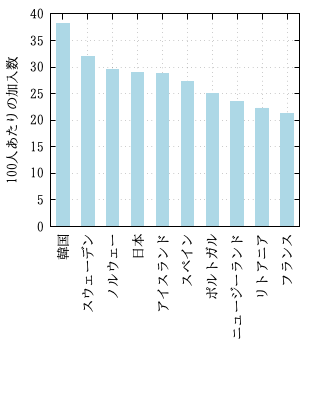
\includegraphics[width=0.6\linewidth]{fig11.png}
    \caption{光ファイバー回線の加入者数（100人あたり）}\label{fig:光ファイバー}
\end{figure}
\section{デジタル競争力ランキング}
国際経営開発研究所（IMD）の調査\cite{imd}によると、表\ref{tbl:デジタル}に示すように、日本のデジタル競争力のランキ
ングは調査対象の64カ国中、総合で28位、知識分野で25位となっている。
\begin{table}[htbp]
    \centering
    \caption{デジタル競争力ランキング(64カ国中)}
    \label{tbl:デジタル}

    \begin{tabular}{|c|c|c|}\hline
        国 & 総合 & 知識 \\
        \hline
        米国 & １位 & ３位 \\
        \hline
        香港 & ２位 & ５位 \\
        \hline
        スウェーデン & ３位 & ２位\\
        \hline
        デンマーク & ４位 & ８位 \\
        \hline
        シンガポール & ５位 & ４位 \\
        \hline
        韓国 & １２位 & １５位 \\
        \hline 
        中国& １５位 & ６位\\
        \hline
        日本 &  ２８位 & 25位\\
        \hline
    \end{tabular}
\end{table} 
\section{考察}
\begin{itemize}
    \item アメリカは国土も広くお金もたくさんあるので、常に最先端を走るここができる。
    \item 日本は今デフレでお金が不足してるため、最先端を走れない時がある。
    \item シンガポールはIT分野に多額にお金をかけているので、ランキングが高い。
\end{itemize}


% ここから本文
% 節見出し: \section{}
% を使う

% 本文(1)
%  参考文献の参照: \cite{}
%  図番号の参照： \ref{}
% を使う
% 文献データベースのキーワードは oecd と imd
% になっている．

% 図の挿入
% \includegraphics{}
% を
% \begin{figure}[htbp]
% \end{figure}
% で囲み
% \caption{}
% で図のタイトルを入れる．
% \label{}
% を使って図番号が参照できるようにする
% また，
% \centering
% で図が中央に来るようにする

% ーーー
% 節見出し(2)

% 本文(2)

% 表の挿入
% \begin{tabular}
% \end{tabular}    
% による表の記述を 
% \begin{table}[htbp]
% \end{table}
% で囲み
% \caption{}
% で表のタイトルを入れる．
% \label{}
% を使って表番号が参照できるようにする
% また，
% \centering
% で表が中央に来るようにする

% ーーー
% 見出し(3)
% 考察
%
% \begin{itemize}
% \end{itemize}
% を使って箇条書きで記述する

% ここに参考文献が入る
%
\bibliographystyle{junsrt}
\bibliography{exercise.bib}

\end{document}